\documentclass[tikz,border=10pt]{standalone}
\usepackage{tikz}
\usetikzlibrary{shapes.geometric, arrows, positioning, fit, backgrounds, calc}
\usepackage{xcolor}

% Colores
\definecolor{rfblue}{RGB}{41, 128, 185}
\definecolor{dspgreen}{RGB}{39, 174, 96}
\definecolor{nnred}{RGB}{192, 57, 43}
\definecolor{outgray}{RGB}{127, 140, 141}

\begin{document}
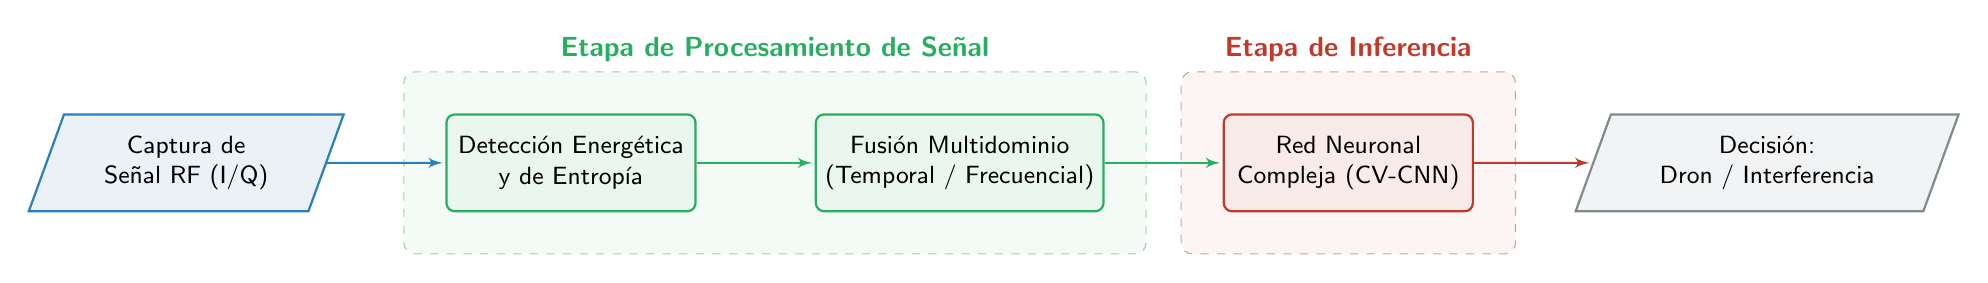
\begin{tikzpicture}[
    auto,
    block/.style={
        rectangle,
        draw=black!80,
        thick,
        fill=white,
        align=center,
        rounded corners=3pt,
        minimum height=3.5em,
        minimum width=9em,
        font=\sffamily\small
    },
    line/.style={draw, thick, -latex', shorten >=1pt},
    io/.style={
        trapezium,
        trapezium left angle=70,
        trapezium right angle=110,
        draw=black!80,
        thick,
        fill=white,
        align=center,
        minimum height=3.5em,
        font=\sffamily\small
    }
]

    % Nodos
    \node [io, fill=rfblue!10, draw=rfblue] (input) {Captura de\\Señal RF (I/Q)};
    
    \node [block, fill=dspgreen!10, draw=dspgreen, right=1.5cm of input] (detector) {Detección Energética\\y de Entropía};
    
    \node [block, fill=dspgreen!10, draw=dspgreen, right=1.5cm of detector] (preprocessing) {Fusión Multidominio\\(Temporal / Frecuencial)};
    
    \node [block, fill=nnred!10, draw=nnred, right=1.5cm of preprocessing] (cnn) {Red Neuronal\\Compleja (CV-CNN)};
    
    \node [io, fill=outgray!10, draw=outgray, right=1.5cm of cnn] (output) {Decisión:\\Dron / Interferencia};

    % Conexiones
    \path [line, draw=rfblue] (input) -- (detector);
    \path [line, draw=dspgreen] (detector) -- (preprocessing);
    \path [line, draw=dspgreen] (preprocessing) -- (cnn);
    \path [line, draw=nnred] (cnn) -- (output);

    % Background Boxes
    \begin{pgfonlayer}{background}
        \node[fit=(detector)(preprocessing), fill=dspgreen!5, rounded corners, draw=dspgreen!50, dashed, inner sep=15pt, label={[font=\sffamily\bfseries, text=dspgreen]above:Etapa de Procesamiento de Señal}] (dspbox) {};
        
        \node[fit=(cnn), fill=nnred!5, rounded corners, draw=nnred!50, dashed, inner sep=15pt, label={[font=\sffamily\bfseries, text=nnred]above:Etapa de Inferencia}] (nnbox) {};
    \end{pgfonlayer}

\end{tikzpicture}
\end{document}
